% !TEX encoding = UTF-8
% !TEX TS-program = pdflatex
% !TEX root = ../tesi.tex
% !TEX spellcheck = it-IT

%**************************************************************
\chapter{L'azienda e gli stage}
\label{cap:stage}
%**************************************************************

\intro{Il presente capitolo è dedicato al rapporto dell'azienda 
	con gli stage in collaborazione con l'Università degli Studi di Padova. Nello 
	specifico presento: l'ambito, le motivazioni, obiettivi 
	aziendali e personali, e i vincoli del mio progetto di stage.
}

%**************************************************************
\vspace{20pt}
Lo spirito dell'azienda è investire costantemente sui propri dipendenti e 
soddisfare i bisogni tecnologici del mercato con le giuste competenze. 
I dipendenti tecnici dedicano parte della propria giornata di lavoro in 
approfondimenti tecnologici e attività di laboratorio. 

A supporto dell'attività di laboratorio è stato installato un ambiente virtuale. 
Avere a disposizione un simile environment permette di sperimentare con: nuove 
tecnologie, integrazione di sistemi ed ecc. Inoltre, permette di mettere a 
disposizione degli stagisti un infrastruttura dedicata ai loro progetti di 
stage. Oltre alla virtualizzazione è possibile sperimentare nei 
seguenti ambiti: storaging, networking e security. Temi comuni 
di approfondimento specializzante sono: Cloud, Machine Learning e Analytics. 

Di recente, l'Azienda ha concluso una partnership strategica con AWS, il provider
di cloud pubblico. L'accordo di collaborazione permetterà a IKS di portare 
molte delle proprie soluzioni sul Cloud e beneficiare delle sue 
peculiarità: elasticità, flessibilità nella gestione di infrastrutture ed ecc. 

Per monitorare e prevenire le frodi bancarie IKS ha sviluppato alcune soluzioni. 
Queste usano tecniche sofisticate di Machine Learning e analisi dei log. 
Inoltre, è in corso un progetto per il loro rilascio come servizio. 
In questo modo gli utilizzatori avranno la possibilità di integrare la soluzione 
nei propri sistemi e monitorare il flusso delle transazioni bancarie in tempo
reale.  

Ogni anno l'azienda partecipa a StageIT: un evento completamente dedicato agli 
studenti universitari dei Corsi di Laurea in Scienze e Ingegneria Informatica.
Infatti, quest'evento è un'opportunità per lo studente di mettersi in contatto con 
le realtà aziendali e per queste ultime di conoscere i talent più da vicino. 
Durante l'evento è previsto anche un concorso che promuove il miglior progetto 
di stage. In generale su un'insieme di progetti effettuati nell'edizione
precedente dell'evento vengono scelti un sotto insieme ristretto di finalisti
da una commissione orientata alla promozione dell'innovazione. 

Il vincitore, invece, è scelto dagli studenti in tempo reale durante l'evento. Il premio del vincitore è un buono d'acquisto del valore di 500 Euro.

\section{Il valore aggiunto di uno stagista}

IKS è un partecipante attivo a StageIT e annualmente propone fino a 
6 progetti di stage. Questi non sono verticali su un'unica 
tematica ma usualmente coinvolgono temi come: 

\begin{itemize}
	\item Sviluppo di applicazioni basate su web, \gls{cloud}, mobile 
	      o migrazione su \gls{cloud}/mobile di applicazioni tradizionali;
	\item Progettazione di ambienti, metodologie e strumenti di 
	      sviluppo software.
\end{itemize}

Lo stagista è una risorsa importante per l'azienda. Esso viene visto 
come un portatore di novità. In principio, lo stagista è impiegato su progetti 
di sperimentazione. I quali hanno come obiettivo: lo studio e l'analisi 
di fattibilità dell'integrazione delle soluzioni nell'offerta commerciale dell'azienda. 

Per l'intera durata dello stage, lo stagista si emerge in un ambiente di lavoro il più possibile vero simile alla realtà aziendale. Questo permette al tutor esterno di analizzare più da vicino il candidato in stage. E alla fine dello stage allo stagista può essere proposta un'offerta d'assunzione. 

L'Azienda, grazie al contributo degli stagisti, si allinea con i temi di ricerca 
universitari e con le tendenze tecnologiche del momento sul mercato internazionale.

\section{Alcuni temi di stage}
\subsection{AIOps e Machine Learning}
Il progetto di stage tratta l'integrazione del Machine Learning con 
strumenti di Application Performance Monitoring. L'obiettivo dello 
stage è sperimentare integrando diverse soluzioni in questo ambito e 
studiarne il prodotto finale. Una conseguenza critica di questo progetto 
è lo sviluppo di un pensiero critico per affrontare le più difficili sfide 
del monitoraggio di applicazioni e infrastrutture. 

Il presente progetto si colloca in ambito del \textit{application and performance monitoring} che è un servizio offerto dall'azienda al supporto della governance IT.


\subsection{DevOps Automazione}
L'automazione è fondamento di ogni realtà aziendale contemporanea. Infatti, 
il numero di macchine da gestire spesso non è piccolo. Per semplificare i 
compiti di gestione si devono utilizzare strumenti di configurazione e
automazione. Queste tecnologie permettono di automatizzare tutte le operazioni 
manuali che un sistemista spesso compie durante le attività di manutenzione 
giornaliere. L'obiettivo di questo progetto è l'integrazione di alcuni strumenti che semplificano il \gls{patching} dei server e sperimentare con nuove tecnologie del settore.
Il presente progetto si colloca nell'ambito del \textit{system management}. 

\subsection{Sviluppo moduli evolutivi in ambito antifrode}
IKS ha grande esperienza in ambito della sicurezza informatica bancaria. 
Come prodotto risultate di questa esperienza è SMASH. L'obiettivo dello 
stage è estendere il prodotto con qualche funzionalità di monitoraggio di 
azioni sospette. Oltre allo sviluppo di moduli evolutivi lo stagista ha 
la possibilità di apprendere delle competenze forti nell'ambito della 
sicurezza informatica. 
La presente proposta di stage è un progetto inter business unit dell'azienda. 
Esso si colloca nell'ambito dello sviluppo di prodotti software e della sicurezza
informatica nel settore bancario.


\section{Il progetto proposto}
\subsection{Motivazioni}

E' sempre più comune nelle realtà aziendali l'impiego dell'approccio agile nelle attività di lavoro giornaliero. Infatti, questo approccio promuove la comunicazione in generale e focalizza l'attenzione di tutti i stakeholder sul valore finale, per esempio di un prodotto software oppure di una strategia di mercato, che deve essere garantito. 

Se gli sviluppatori hanno come obiettivo primario lo sviluppo di un prodotto software, i professionisti dell'IT hanno come priorità la sua garanzia di servizio e manutenzione periodica. 

\begin{figure}[htbp]
	\begin{center}
		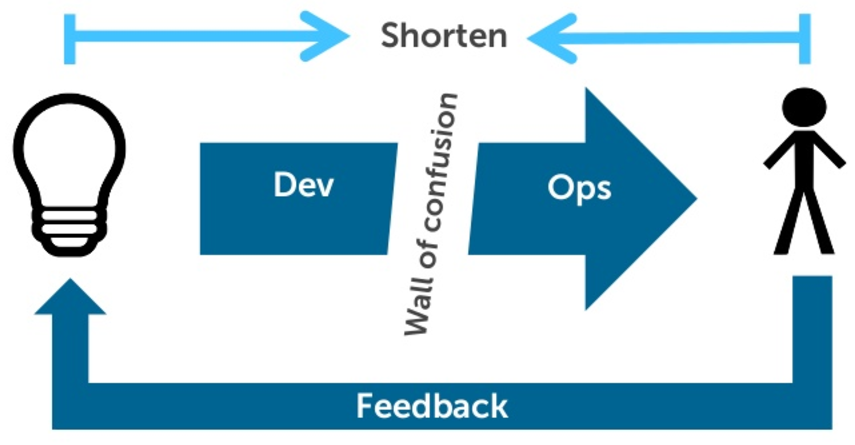
\includegraphics[height=4cm]{devops-wc}
		\caption{Sia gli sviluppatori che i professionisti IT sono portatori di valore: un feedback che coinvolge ambe le parti è essenziale. Immagine tratta da: http://bit.ly/2rM9lBQ.}
	\end{center}
\end{figure}


Tra i due gruppi esiste un muro di incomprensione. Questo fenomeno è dovuto alla mancanza di comunicazione ed interazione. In caso di eventuali problemi che possono incorrere dopo il rilascio del prodotto software è sola responsabilità dei professionisti IT rimuoverli e riportare il prodotto software in uno stato di operatività non a rischio.

Un simile scenario per un'azienda informatica che deve affrontare un numero elevato di rilasci giornalieri non è accettabile. A questo scopo si è creato un movimento culturale, chiamato DevOps, orientato all'unione degli sviluppatori e sistemisti. L'unione promuove un cambio di mentalità, creazione di nuove competenze e sviluppo di nuovi strumenti che diminuiscano la distanza tra le due realtà. 

Il DevOps ha conseguenze più profonde del semplice cambio culturale. Un'azienda che 
approccia il DevOps affronta un cambiamento interno che ripensa il proprio modello di qualità. I benefici del cambio sono i seguenti: maggiore innovazione, agilità nel cogliere i bisogni di mercato del momento, flessibilità nel gestire il cambiamento e maggior qualità di prodotto e processo.

Una tipica rappresentazione del ciclo di vita DevOps è come segue in figura. 

\begin{figure}[htbp]
	\begin{center}
		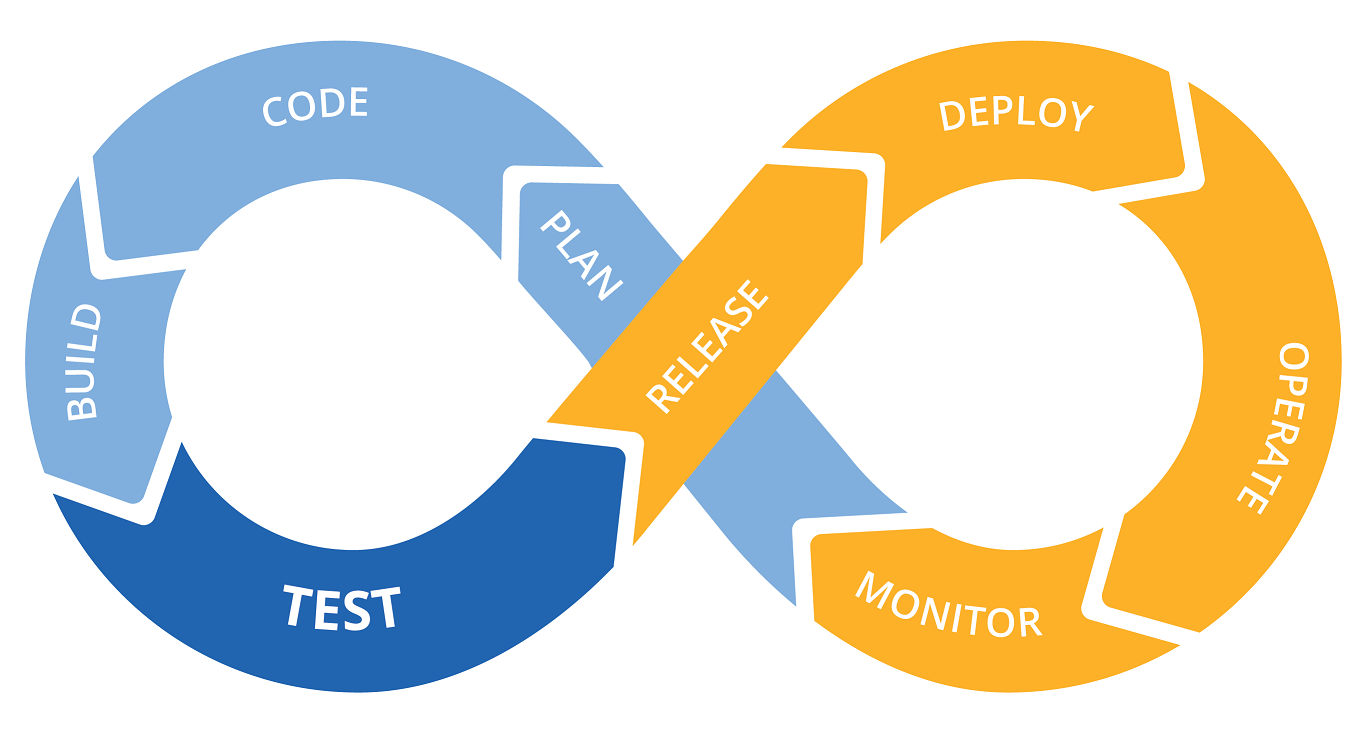
\includegraphics[height=4cm]{devops-pipeline}
		\caption{Il DevOps abilità l'automazione del processo di rilascio del software e i cambi dell'infrastruttura IT. Immagine tratta da: http://bit.ly/2rsw9nm.}
	\end{center}
\end{figure}

L'abilità di poter cambiare quando necessario in modo agile è un beneficio notevole 
per le aziende; in questo modo i dipendenti sono impiegati nel creare solo valore aggiunto per l'azienda e il mercato. Invece, la gestione dell'infrastruttura è disciplinata, sistematica e standardizzata. Con un approccio standardizzato e ben strumentalizzato è sempre più difficile individuare server nomadi. Può succedere che in caso di operazioni sofisticate di manutenzione un server scompaia dall'orizzonte di visibilità. Se siamo in ambiente Cloud questo risulta in costi in eccesso. Se siamo in ambiente virtualizzato questo risulta in riduzione della capacità complessiva di calcolo. 

Sebbene il DevOps possiede uno scopo più ampio, il \textit{continuous delivery} è un approccio che promuove l'automazione di tutti i processi che vengono coinvolti 
durante il rilascio di un prodotto software. Il \textit{continuous delivery} permette di abbreviare i tempi di rilascio e aumentarne il loro numero, e migliorare la gestione del cambiamento.

Essere veloci nel \textit{delivery} di un prodotto software non è sufficiente. E' necessario prevedere una \textit{pipeline} di \textit{deploy} per il software che si vuole portare nell'ambiente di produzione. L'ambiente direttamente esposto all'uso dei clienti. Automatizzare questo passaggio implica minor intervento manuale e minor numero di errori e conseguentemente maggior rigore nelle attività complessive coinvolte. 

L'utilizzo di \textit{application container} permette di confezionare le applicazioni in un'unità singola che contiene anche le sue dipendenze. Confezionare in questo modo le applicazioni rende facile lo scambio di artefatti tra i diversi gruppi. Di conseguenza lo stesso artefatto creato da uno sviluppatore verrà consegnato al verificatore che attuerà il \textit{testing} di quel particolare prodotto con una specifica versione e sistemista che ne prevederà il suo successivo rilascio.

Un esempio di strumento di containerizzazione è LXC (Linux Kernel Container), Docker ed ecc. Il primo è un progetto che permette il supporto dei container a livello del kernel Linux. Docker è un'altra soluzione di containerizzazione. Le prime versioni Docker offrivano un insieme di API per interagire con LXC, ora Docker offre una propria soluzione di containerizzazione completamente indipendente da quella Linux. 

Con la containerizzazione segue un'estrema facilità nel gestire le applicazioni durante il loro intero ciclo di vita. 

Il cambio di filosofia è percepibile anche al livello architetturale dei prodotti software. In un ambiente dinamico caratterizzato dall'automazione, verifiche e deploy automatici le classiche architetture software non riescono a beneficiare di questa flessibilità. A questo scopo i microservizi rappresentano uno stile architetturale in sintonia con la filosofia delle \textit{pipeline} Unix: ogni microservizio implementa una sola funzionalità - basso accoppiamento.

\begin{figure}[htbp]
	\begin{center}
		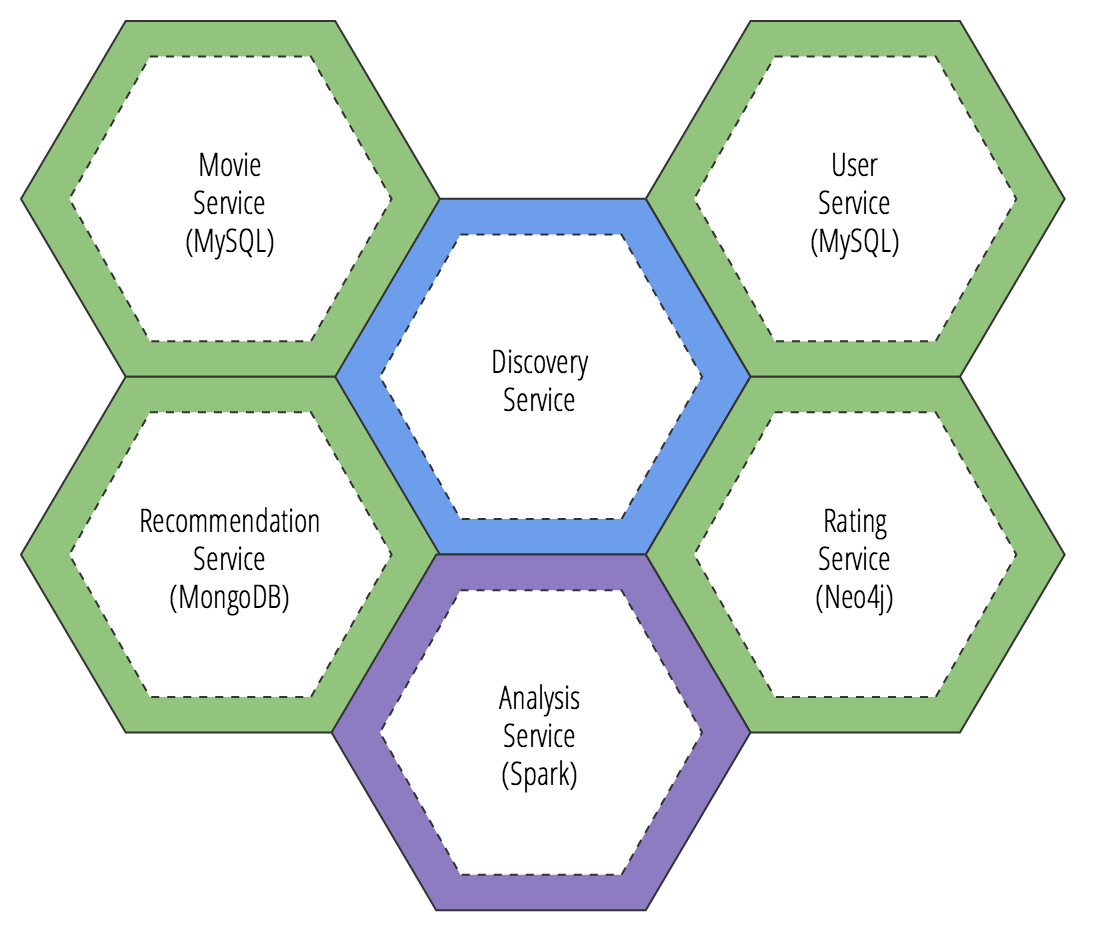
\includegraphics[height=5cm]{microservice-example}
		\caption{Esempio di un sistema a microservizi. Immagine tratta da: http://bit.ly/2qNXKxj.}
	\end{center}
\end{figure}

In figura è possibile notare diversi microservizi. Ciascuno ha una responsabilità
ben definita. Questi possono comunicare tra di loro. Per garantire un alto disaccoppiamento tra i servizi è necessario introdurre un microservizio di servizio, chiamato \textit{Service Discovery}, utilizzato come un DNS (Domain Name System). In questo modo i microservizi possono coesistere nello stesso ambiente e comunicare solo quando necessario senza conoscersi direttamente. Inoltre, i microservizi ottengono un'indipendenza dal luogo di esecuzione. Se un microservizio X in esecuzione su una macchina A migra per eseguire su una macchina B allora un microservizio Y che vuole comunicare con X deve contattare il \textit{Service Discovery} per ottenere l'indirizzo di X. L'effetto che si ottiene è un alto tasso di mobilità dei servizi.  

E' usuale incapsulare un microservizio in un container software. In questo modo 
ogni microservizio diventa un'unità funzionale indipendente e nello stesso ambiente possono coesistere due o più copie dello stesso servizio eliminando l'interferenza dell'uno sull'altro. 
Per aumentare la capacità di robustezza e affidabilità di un microservizio sarà 
sufficiente scalare in orizzontale creando una copia aggiuntiva del microservizio che soffre delle proprietà precedentemente citate. 
Il traffico in ingresso sarà bilanciato con qualche politica di distribuzione del carico ai due microservizi attivi tramite un \textit{Load Balancer}. 

\begin{figure}[htbp]
	\begin{center}
		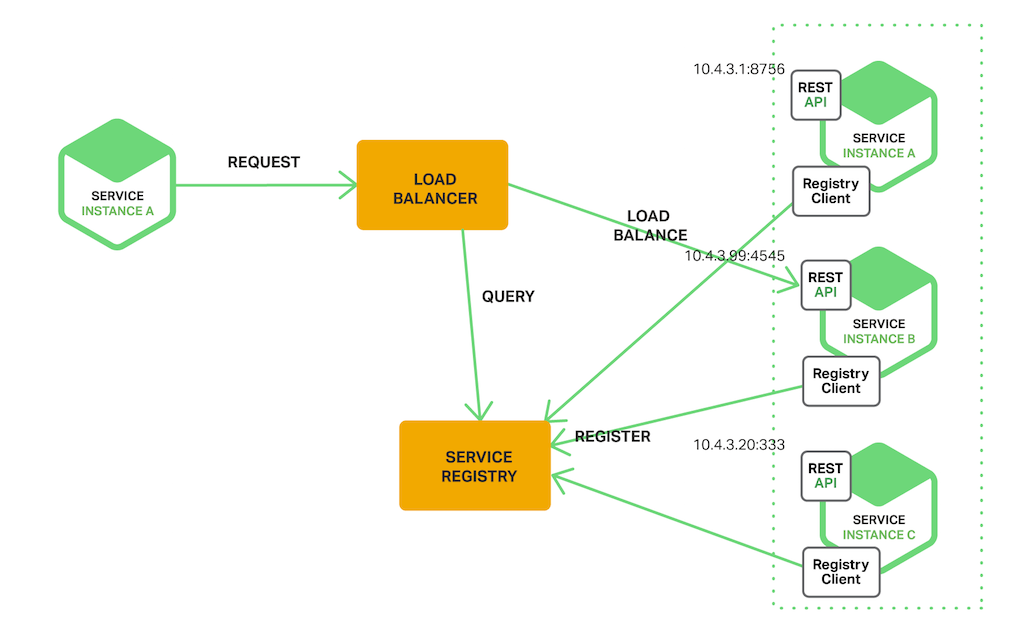
\includegraphics[height=6cm]{richardson-microservices}
		\caption{I microservizi permettono di scalare orizzontalmente per reggere ai più esigenti carichi di lavoro. Immagine tratta da: http://bit.ly/2qI50LR.}
	\end{center}
\end{figure}

I microservizi semplificano di molto l'applicazione complessiva scomponendo il prodotto in sotto applicazioni indipendenti; complicano l'applicazione nel complesso perché vengono aggiunte componenti nuove e il traffico inter microservizio diventa molto più difficile da gestire.

Si aprono nuove sfide sia per gli sviluppatori che per i sistemisti. 
E queste sfide caratterizzano il contratto di collaborazione tra i due gruppi. 


%%% ------------------------------------------------------------------------------

%%% -------------------------------------------------------------------------------

\subsection{Obiettivi aziendali}

Un team interno di IKS ha sviluppato una soluzione di Executive e Malware Dashboard
basata sullo stack applicativo: Elasticsearch, Logstash e Kibana.
 
L'obiettivo principale del mio progetto di stage è la containerizzazione della 
soluzione precedentemente implementata e garantire l'alta affidabilità delle dashboard. 

Inoltre, tramite l'utilizzo della tecnologia dei container applicativi l'azienda 
ha l'obiettivo di individuare una soluzione architetturale dell'applicativo affinché sia portabile su ambienti come Cloud, macchine virtuali e/o fisiche, e sul portatile dello sviluppatore. 

Oltre alla portabilità dell'applicativo è necessario garantire anche la portabilità dell'infrastruttura che ospita l'applicativo per l'esecuzione.

Con la garanzia di alta portabilità il team di gestione dell'infrastruttura potrà gestire lo stesso ambiente in contesti differenti e affini a scopi diversi in modo univoco. 


\subsection{Obiettivi personali}
Come attività preliminare alla ricerca di un progetto di stage per la Laurea ho 
attuato uno studio individuale di mercato. Lo scopo era capire: tendenze 
tecnologiche, architetturali e metodologiche. Se da un lato le mie ricerche 
hanno cercato di cogliere le novità del momento, dall'altro a livello personale 
queste erano mirate alla ricerca di un contesto in cui potermi applicare e maturare. 

Con il presente progetto gli obiettivi personali erano:

\begin{itemize}
	\item Apprendere conoscenze e competenze in ambito di:
		\begin{itemize}
			\item Virtualizzazione basata sulla tecnologia a container; 
			\item Sistemi distribuiti;
			\item Amministrazione di sistema Linux;
	    \end{itemize}
	\item Acquisire esperienza pratica nella gestione delle reti di calcolatori in ambito dei sistemi, nello specifico le reti definite in modo programmatico per le tecnologie orientate alla containerizzazione; 
	\item Acquisire esperienza nell'analisi, progettazione e implementazione di sistemi orientati ai microservizi;
	\item Famigliarizzare con la piattaforma Kubernetes e i principi del \gls{cloud}.
\end{itemize} 

\section{Piano di lavoro}
\label{sec:piano-di-lavoro}
Il piano di lavoro è stato pianificato per un totale di 300 ore complessive. Il 
contenuto del piano è stato presentato in un documento di cui una copia è stata 
consegnata all'Ufficio degli Stage presso l'Ateneo dell'Università di Padova, 
una seconda copia è stata consegnata al tutor interno e l'ultima copia 
controfirmata dall'ufficio stage dell'Università è stata consegnata all'azienda. 
Il piano è stato strutturato in tre fasi il cui contenuto presento di seguito:
\begin{itemize}
\item Fase 1 - Formazione  (56 ore)
	\begin{itemize}
		\item Docker: la tecnologia per la containerizzazione;
		\item Kubernetes: la tecnologia per l'orchestrazione;
		\item ELK: lo stack applicativo;
		\item Verifiche delle competenze acquisite;
	\end{itemize}
\item Fase 2 - Analisi e progettazione  (56 ore)
	\begin{itemize}
		\item Analisi delle funzionalità della soluzione non containerizzata di dashboard;
		\item Analisi delle modalità di containerizzazione delle componenti;
		\item Analisi delle modalità di \gls{deployment};
		\item Progettazione delle modalità di verifica della non regressione;
		\item Progettazione architetturale della soluzione; 
		\item Progettazione della modalità di \gls{deployment};
		\item Documentazione;
	\end{itemize}
\item Fase 3 - Implementazione  (188 ore)	
	\begin{itemize}
		\item Installazione e configurazione dell'orchestratore;
		\item Implementazione della soluzione in un contesto con e senza orchestratore;
		\item Verifica di non regressione;
		\item Documentazione.
	\end{itemize}
\end{itemize}

\section{Vincoli}
\subsection{Vincoli temporali}
Lo stage è durato 8 settimane per un complessivo di 310 ore di lavoro. Ho lavorato a tempo pieno con il seguente orario: 9.00-18.00. Con la pausa pranzo di 1 ora dalle 12.30 alle 13.30. Come stabilito nel PdL (Piano di Lavoro) le attività sono state strutturate in tre fasi. Ogni fase ha coinvolto attività mirate al raggiungimento di specifici obiettivi. Per maggior dettaglio sul contenuto del PdL riferire la \hyperref[sec:piano-di-lavoro]{sezione Piano di Lavoro}.

\subsection{Vincoli tecnologici}

Fin dal primo giorno di lavoro l'azienda mi ha fornito un portatile dedicato per l'itero periodo di stage. Inoltre, mi è stato vietato di collegare alla rete aziendale qualsiasi dispositivo personale. Inoltre, il portatile di lavoro non poteva essere portato a casa.
Per comunicare internamente sono stati utilizzati strumenti di messaggistica istantanea, come Skype, per comunicazioni informali e la posta elettronica.

Oltre a questo vincolo, a livello tecnologico sono state fissate le seguenti tecnologie:

\begin{itemize}
	\item CentOS7: il sistema operativo installato sulle macchine di laboratorio. CentOS7 è la versione open source di RHEL7 (Red Hat Enterprise Linux versione 7);
	\item Docker: è uno strumento che permette in modo estremamente facile la creazione, il deploy e l'esecuzione di applicazioni utilizzando la tecnologia a container. In questo modo l'attenzione dell'utente è focalizzata su questioni diverse dall'installazione e configurazione dell'applicazione. 
	L'architettura di Docker segue in figura. 
	
	\begin{figure}[htbp]
		\begin{center}
			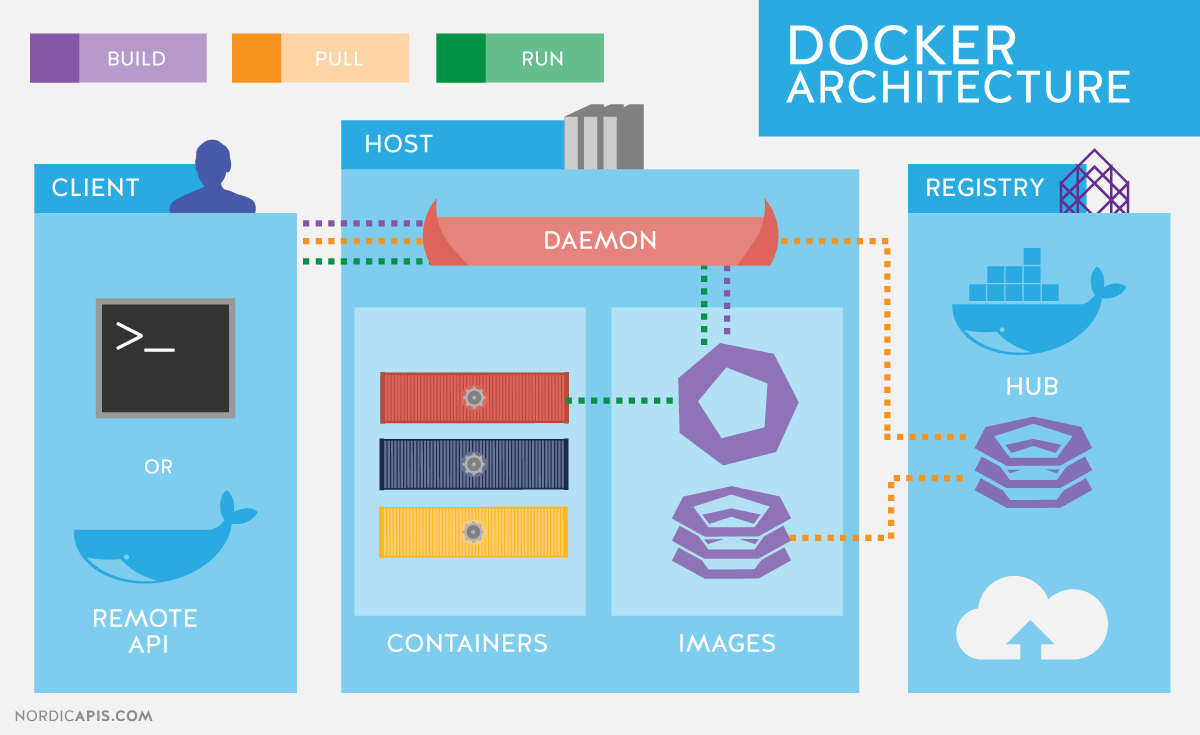
\includegraphics[height=6cm]{docker-architecture}
			\caption{Le parti costituenti la piattaforma Docker sono: il demone, il client e il registry Docker. Immagine tratta da: http://bit.ly/2rmkt7g.}
		\end{center}
	\end{figure}
	
	Le componenti architetturali costituenti la piattaforma Docker sono il:
	demone, client e registry. Si può notare che l'architettura di alto livello è 
	un architettura client/server. Il server di Docker è il demone che ha la responsabilità di gestione dei container sulla macchina locale. Mentre il client si interfaccia tramite un'interfaccia REST al demone e permette di interagire in modo agile con i container, creare reti virtuali, gestire i dati che devono essere condivisi tra i container e il file system locale della macchina. Infine, il registry di Docker è una repository che può essere pubblica o privata e ha la responsabilità di abilitare la condivisione di immagini utili alla creazione dei container. Come modello mentale, in relazione con il paradigma ad oggetti, è possibile paragonare le immagini Docker a classi che devono essere istanziate per la creazione di oggetti, ovvero container. 
	
	Per favorire il libero scambio di immagini Docker, l'azienda Docker Inc ha 
	messo a disposizione degli utenti un hub completamente gratuito. Nella versione privata di una repository è disponibile il servizio di \textit{scanning} delle immagini per individuare le vulnerabilità di sicurezza. 
	
	Quando si esegue il comando run tramite la CLI di Docker il demone controlla che l'immagine da usare per la creazione del container sia presente in locale. In caso affermativo il container viene creato e messo in esecuzione, altrimenti il demone scarica l'immagine dal registry e al termine del \textit{download} istanzia il container;
	\item Kubernetes: è un sistema open source per automatizzare il deploy, la scalabilità e gestione di applicazioni containerizzate. La tecnologia è un 
	prodotto risultante da 15 anni di esperienza in Google con i container. Essa garantisce la portabilità delle applicazioni e l'indipendenza dall'ambiente fisico di esecuzione.
	
	Kubernetes è un sistema distribuito e il modello architetturale è master/slave.
	
	\begin{figure}[htbp]
		\begin{center}
			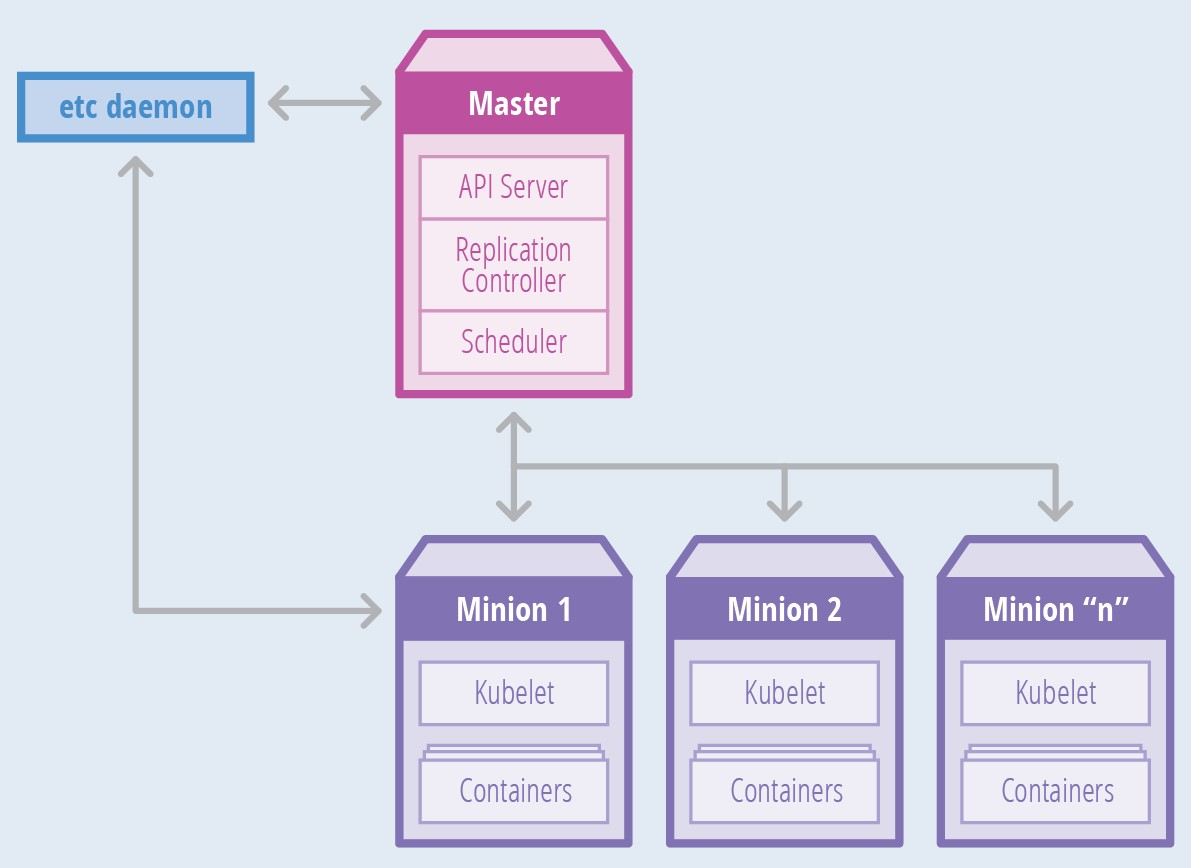
\includegraphics[height=6cm]{kube-architecture}
			\caption{Le componenti architetturali di Kubernetes sono: API server, Scheduler, Replication Contoller, Kubelet, Kube proxy, Database Etcd. Immagine tratta da: http://bit.ly/2s4eKUR.}
		\end{center}
	\end{figure}
	
	Il master è un pannello di controllo del sistema K8s (Kubernetes). La sua responsabilità è gestire il \textit{workload} a container. Inoltre, esegue le componenti critiche del sistema: il database chiave valore ad alta consistenza etcd, il gestore delle repliche per la scalabilità orizzantale - replication controller e lo scheduler.  
	
	La componente slave esegue il carico di lavoro. Essa comunica solo con il master e salva le informazioni di servizio tramite il API server nel database etcd. 
	
	Ogni componente master e slave eseguono un agente locale chiamato Kubelet. Il compito dell'agente è quello di collegare le varie componenti e comunicare con il demone Docker. 
	
	Infine, il Kube proxy è la componente che gestisce il traffico di rete dell'intera infrastruttura. 
	
    Kubernetes, essendo un sistema fin dall'inizio pensato per essere componibile 
    si può integrare bene con soluzioni di terzi parti, come per esempio: diverse soluzioni per lo storage, diversi plugin per la rete ed ecc;
	
	\item Elasticsearch, Logstash e Kibana: Le tre componenti sono comunemente conosciute con l'acronimo ELK.  Esse vengono utilizzate insieme come una soluzione open source in progetti che hanno forti esigenze di ricerca e analisi di dati. Elasctisearch è il cuore dello stack applicativo. Esso è un database NoSQL e distribuito implementato in Java. Orientato all'immagazzinamento di dati non strutturati permette di effettuare ricerche complesse impiegando millisecondi contro i secondi necessari utilizzando un classico DB SQL. Kibana, invece, è la componente dello stack che offre la funzionalità di visualizzazione dei dati presenti in Elasticsearch. Una peculiare caratteristica di Kibana è l'interfaccia di creazione di cruscotti. Essendo la soluzione nativa di visualizzazione per Elasticseach, Kibana permette di sfruttare questa integrazione per esprimere ricerche molto complesse e visualizzarle a video tramite effetti grafici accattivanti. Infine, Logstash è la componente di estrazione, trasformazione e caricamento dei dati dalla sorgente in Elasticsearch. Con Logstash risulta semplice filtrare l'informazione utile per l'analisi dei dati ed eliminare il rumore di fondo. Essendo uno strumento implementato in Java offre un insieme ricco di strumenti di terzi parti che arricchiscano ulteriormente il suo insieme di funzionalità. Per esempio, tramite uno plugin esterno è possibile programmare Logstash a interagire con le API del social network Twitter per cercare l'informazione che soddisfa dei particolari criteri di ricerca. 
	Dal punti di vista architetturale la soluzione ELK è flessibile e permette di scalare orizzontalmente in proporzione al carico di lavoro. 	
\end{itemize}

Inizialmente sono state fissate anche le rispettive versioni delle componenti 
sopra citate. Tuttavia, nel corso dello stage ho realizzato che bloccare l'evoluzione di un'infrastruttura può comportare qualche problema nel futuro. A questo scopo ho predisposto un ambiente tollerante agli aggiornamenti e che si auto aggiorna. Durante la personalizzazione dell'ambiente mi sono ispirato al principio  \textit{self driven infrastructure} di CoreOS. 
In questo modo gli aggiornamenti delle componenti possono essere effettuati in modo completamente trasparente.

Le immagini per la creazione di container dovevano essere provenienti solo 
dal repository ufficiale di Docker ed essere le immagini ufficiali.